\section{Amplificatori Operazionali Ideali - 16.09.2014}

\subsection{Introduzione}

In questa sessione di laboratorio abbiamo montato due circuiti con amplificatori operazionali. L'obiettivo sarà quello di valutare la risposta di tali circuiti a diversi segnali in input.

\subsection{Materiali}

\begin{itemize} [noitemsep]
\item Oscilloscopio Agilent DSO-X 2002A (bandwidth $\SI{70}{\mega\hertz}$, sample rate $2 GSa/s$);
\item Generatore di tensione continua Agilent E3631A (max $\pm \SI{25}{\volt}$ o $\pm \SI{6}{\volt}$);
\item Generatore di tensione Agilent 33120A con range di frequenza da $\SI{100}{\micro\hertz}$ a $\SI{15}{\mega\hertz}$;
\item Multimetro Agilent 34410A (utilizzato come amperometro e per verificare i valori delle resistenze);
\item Un amplificatore operazionale UA741;
\item Resistenze varie;  
\item Due capacità da $100 \si{\nano\farad}$;
\item Breadboard;
\item Cablaggi vari.
\end{itemize}

\subsection{Premessa sugli amplificatori operazionali ideali}

\begin{wrapfigure}[17]{r}{0.55\textwidth}
 \centering
   {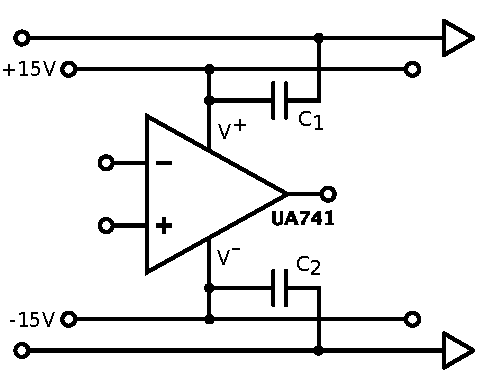
\includegraphics[width=6cm]{../E01/latex/alimentazione.pdf}}
 \caption{Schema circuitale dell'alimentazione dell'op-amp. La tensione di alimentazione è fornita con il generatore di tensione costante, mentre le capacità sono $C_1=C_2=100 \si{\nano\farad}$.}
 \label{gr:costante}
\end{wrapfigure}

Durante l'esperienza considereremo l'amplificatore operazionale come ideale. Questa approssimazione non influisce sui risultati ottenuti visto l'obiettivo della nostra esperienza e le incertezze sui valori considerati. Infatti, assumere un guadagno dell' op-amp $G=\infty$ permette di semplificare l'analisi circuitale. Di seguito sono riportate le cosiddette due regole d'oro:


$\begin{array}{lcl} V_{AB} & = & 0 \\ I_{AB} & = & 0 \end{array}$


La prima equazione ci dice che l'op-amp cerca di portare la differenza di potenziale tra ingresso invertente e non invertente a $0$ modificando la tensione in uscita. La seconda, invece, che l'amplificatore operazionale non lascia passare corrente attraverso i due ingressi.

\'E importante ricordare che si è cercato di limitare al massimo la lunghezza dei cavetti utilizzati per costruire i vari circuiti così da ridurre le resistenze parassite ovviamente presenti non utilizzando conduttori ideali. Viste le assunzioni fatte sull'amplificatore ideale, la loro presenza non è comunque rilevante ai fini della bontà dell'esperimento.




Come vediamo dallo schema circuitale riportato in Fig. \ref{gr:costante} abbiamo alimentato l'op-amp con una tensione di $\pm \SI{15}{\volt}$. Abbiamo inoltre inserito due capacità per eliminare eventuale rumore ($C_1=(112 \pm 1)\si{\nano\farad}$ e $C_2=(95\pm 1)\si{\nano\farad}$).

\subsection{Generatore di corrente}


\begin{wrapfigure}[17]{r}{0.50\textwidth}
  \begin{center}
    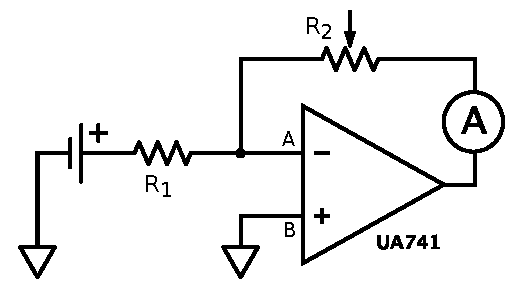
\includegraphics[width=0.35\textwidth]{../E01/latex/c1.pdf}
  \end{center}
  \caption{Schema del generatore di corrente costante costruito con op-amp 741. Come valori abbiamo utilizzato $R1=3.85 \pm 0.01 \si{\kilo\ohm}$ e $V_{gen}=3.85 \si{\volt}$ e $R_2$ variabile.}
\end{wrapfigure}

In questa parte dell'esperienza montiamo un generatore di corrente costante, cioè un dispositivo in grado di erogare una corrente costante indipendentemente dal carico collegato. Per valutare la risposta a diverse resistenze di carico abbiamo dunque utilizzato come $R_2$ una resistenza variabile di tipo \textit{trimmer}. Lo schema circuitale è riportato in figura.



Analizziamo ora il circuito. Dato che B si trova a potenziale di comune, per la prima regola d'oro anche A sarà allo stesso potenziale, che assumiamo nullo. Dunque otterremo:
\begin{equation}
V_{gen}=I R_1
\label{eq:gen_1}
\end{equation}

Poichè non scorre corrente nell'op-amp, la corrente che attraversa $R_2$ è univocamente determinata dalla tensione $V_{gen}$ e da $R_1$.

Possiamo quindi misurare la corrente che scorre nel circuito semplicemente collegando in serie alla resistenza $R_2$ un amperometro. I dati ottenuti sono riportati nella seguente tabella.



%Otteniamo dunque che la tensione di output si modificherà, ad opera dell'OPAMP, in modo da far passare sempre lo stesso valore di corrente attraverso $R_2$; ciò avviene per il fenomeno di retroazione negativa, che ci permette di controllare la tensione di output tramite la resistenza di feedback, che in questo caso è proprio $R_2$, e di ottenere dunque una corrente costante passante per il circuito di feedback. Imponendo l'uguaglianza della corrente possiamo inoltre trovare il valore della tensione di uscita
%$$V_{out}=-\frac{R_2}{R_1} V_{gen}$$

%Durante l'esperienza abbiamo però deciso di misurare la corrente passante per la resistenza piuttosto che la tensione di uscita, ponendo un amperometro fra l'uscita dell'OPAMP e la resistenza di carico $R_2$. Come valore di corrente abbiamo scelto $1 mA$ in modo da discostarci dalla corrente massima in cui l'amplificatore operazionale potrebbe non comportarsi più in maniera ideale ($10/20 mA$); e avendo a disposizione una resistenza $R_1=3.85 \pm 0.01 \si{\kilo\ohm}$, per (\ref{eq:gen_1}), abbiamo utilizzato una tensione continua di $3.85 V$. Di seguito proponiamo alcuni valori sperimentali che confermano la capacità del circuito da noi creato di fornire alla resistenza di carico una corrente costante di $1 mA$ (considerando gli errori sull'ultima cifra come unitari).




\begin{center}
\begin{tabular}{c|c|c|c|c|c|c|c|c}
$R_2$ [$\Omega$] & $0.54(0.01)$ & $35.1(0.1)$ & $412(1)$ & $1020(10)$ & $1990(10)$ & $3070(10)$ & $4170(10)$ & $4710(10)$ \\ 
\hline 
$I$ ($\pm 0.001$) [$\si{\milli\ampere}$] & 1.002 & 1.002 & 1.002 & 1.002 & 1.002 & 1.002 & 1.002 & 1.002 \\ 
\end{tabular}
\end{center}

Come vediamo, il circuito risulta un ottimo generatore di corrente costante anche per resistenze molto variabili. Ricordiamo che comunque, essendo l'alimentazione dell'op-amp limitata a $\pm \SI{15}{\volt}$, il valore di $R_2$ dovrà essere minore di $\frac{|V^-|}{I}$ per far si che la retroazione negativa funzioni correttamente. Nel nostro caso il generatore di corrente ideale funzionerà se $R_2< \SI{15}{\kilo\ohm}$.




\subsection{Sommatore Pesato}

In questa seconda parte dell'esperienza sarà analizzato il sommatore pesato. 

\begin{wrapfigure}[15]{r}{0.55\textwidth}
  \begin{center}
    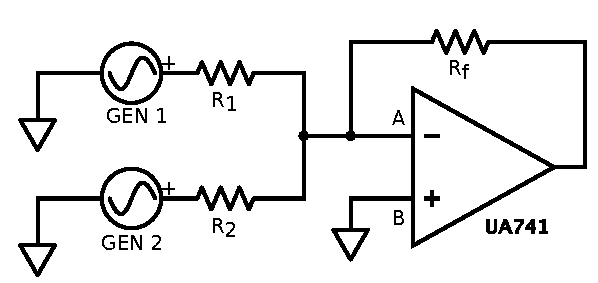
\includegraphics[width=0.40\textwidth]{../E01/latex/c2.pdf}
  \end{center}
  \caption{Schema del sommatore pesato. Come valori abbiamo utilizzato $R_1=(99.9 \pm 0.1) k \Omega$, $R_f=(102.2 \pm 0.1) k \Omega$ e $R_2=(49.8 \pm 0.1) k \Omega$, dove per $R_2$ è stato necessario utilizzare un parallelo di due resistenza da $100 k\Omega$. Come GEN 1 abbiamo utilizzato l'oscilloscopio, mentre per GEN 2 il generatore di forme d'onda. Infine, per valutare la tensione in uscita abbiamo utilizzato l'oscilloscopio.}
\end{wrapfigure}

Analizziamo il circuito. Utilizzando le regole d'oro possiamo immediatemente ottenere le seguenti equazioni:

$\begin{cases} V_A=V_B=0 \\ V_{{GEN}_1} - V_A =I_1 R_1  \\ V_{{GEN}_2} - V_A =I_2 R_2 \\ V_A - V_{out} =(I_1+I_2) R_f \end{cases} $


$$\Rightarrow V_{out}=-R_f \left( \frac{V_{{GEN}_1}}{R_1}+\frac{V_{{GEN}_2}}{R_2}\right)$$

%Si potrebbe dunque definire un peso relativo $\phi_i$ ad ogni segnale dato dal rapporto fra $R_f$ ed $R_{i}$ (con $i=1,2$) e scrivere una formula del tipo

In modo più compatto, $V_{out}=\sum^{2}_{i=1} \varphi_i V_{i}$, dove $\varphi_i=-\frac{R_f}{R_i}$ 

\'E stato deciso di utilizzare $R_f=R_1=100 k\Omega$ e $R_2=50 k\Omega$ così da ottenere semplicemente $\varphi_1=1$ e $\varphi_2=2$.

Presentiamo ora i grafici di alcune forme d'onda in uscita.

\begin{figure}[H]
 \centering
   {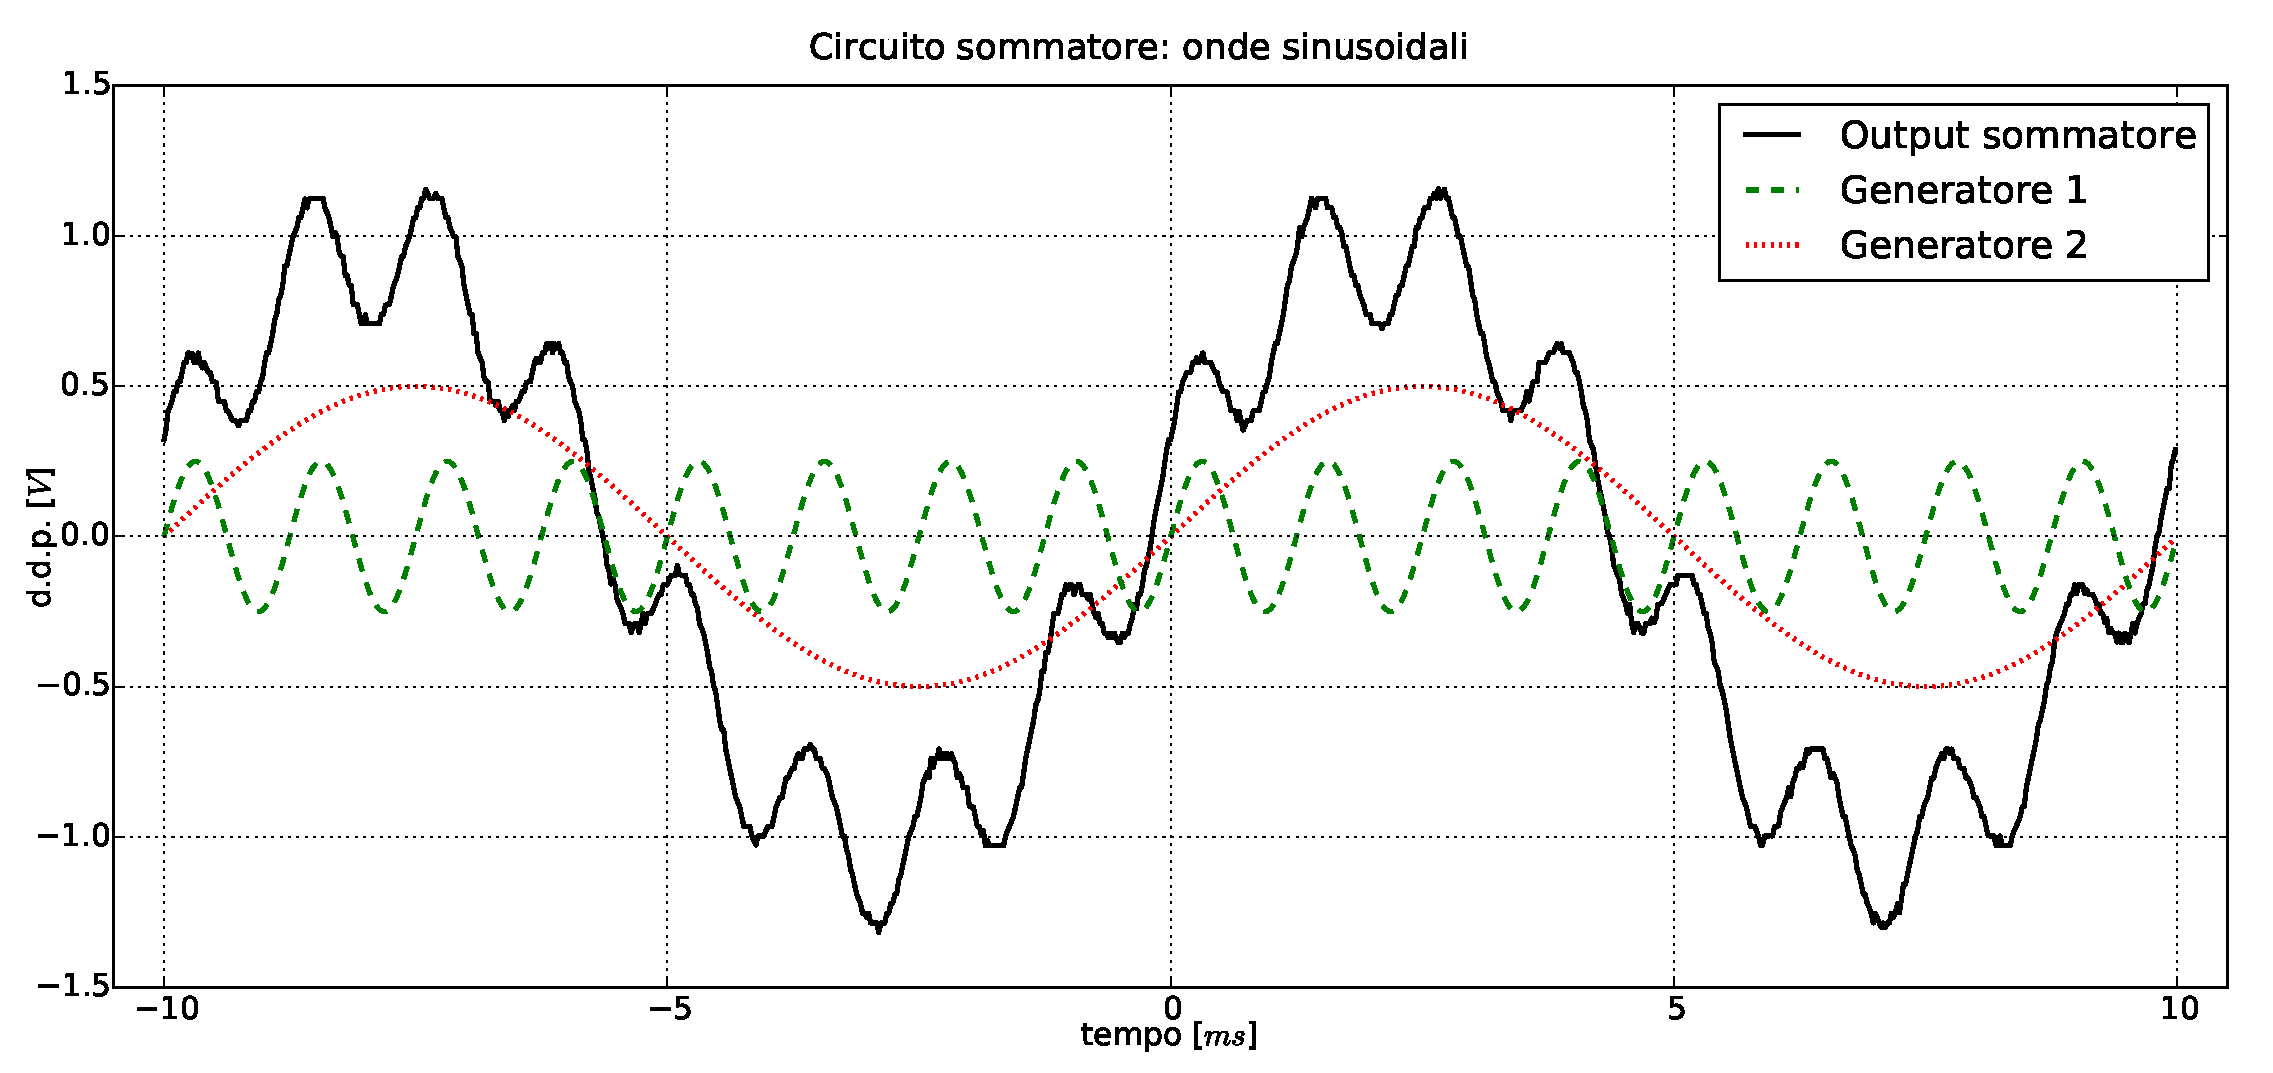
\includegraphics[width=18cm]{../E01/latex/sinsin.pdf}}
 \caption{Grafico della tensione di uscita. Il generatore 1 (generatore dell'oscilloscopio) crea un'onda sinusoidale di $\nu=800 Hz$ e $V^1_{pp}=500 mV$; il generatore 2 (generatore di forme d'onda) crea invece un'onda sinusoidale di $\nu=100 Hz$ e $V^2_{pp}=1000 mV$.}
 \label{gr:onde1}
\end{figure}

Se ricordiamo la formula $V_{out}=\sum^{2}_{i=1} \varphi_i V_{i}$, risulta immediato riscrivere 
\begin{equation}
V_{out}=\frac{V^1_{pp}}{2}\sin(2 \pi \nu_1+ \delta_1)+2\frac{V^2_{pp}}{2}\sin(2 \pi \nu_2+ \delta_2)
\label{eq:batt}
\end{equation}
dove $\delta_1$ e $\delta_2$ sono delle fasi che sono da determinare imponendo $V_{out} \vert_{t=0}=\frac{V^1_{pp}}{2}\sin(\delta_1)+2\frac{V^2_{pp}}{2}\sin(\delta_2)$. 


\begin{figure}[H]
 \centering
   {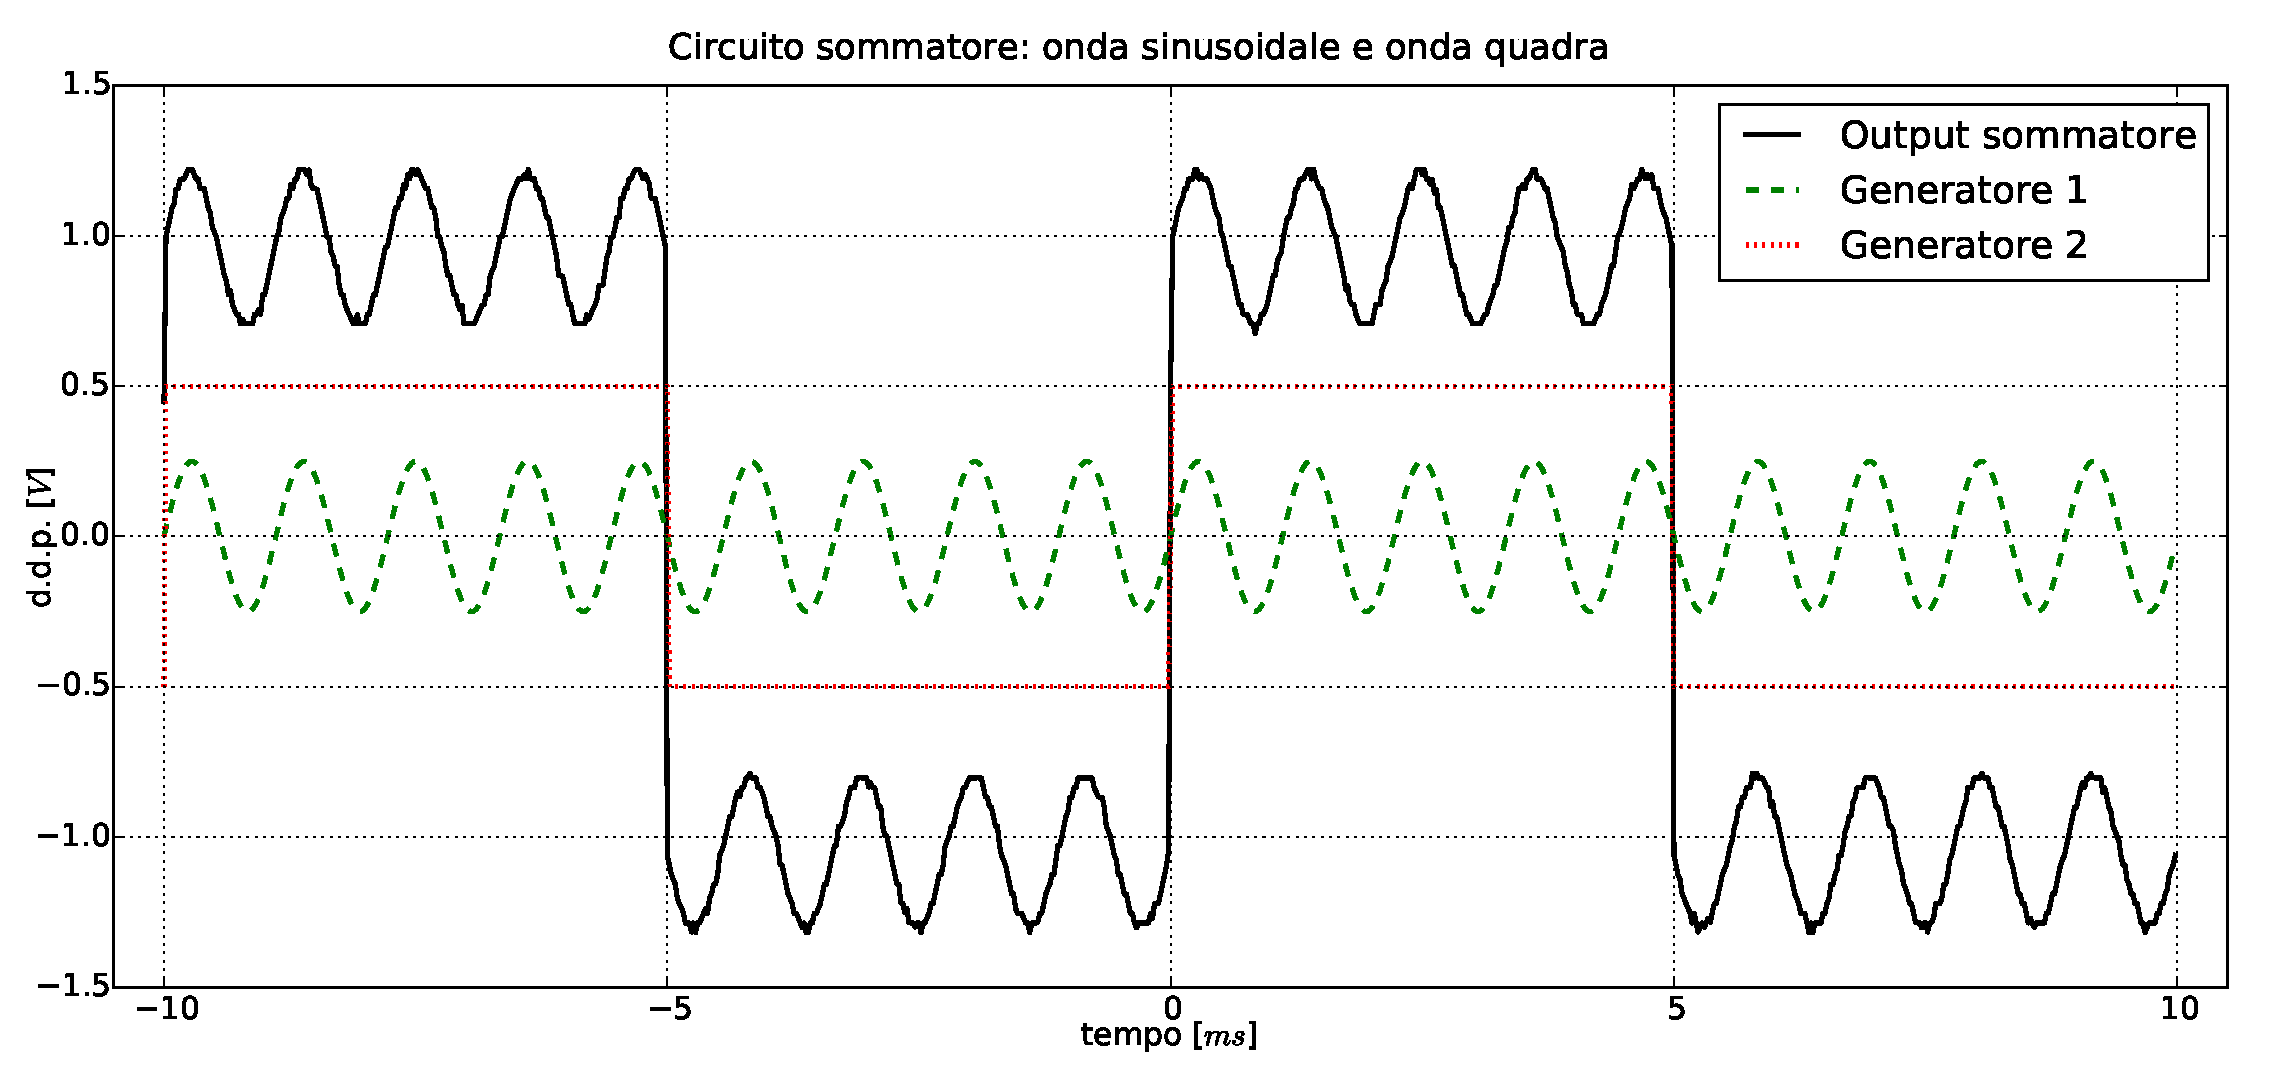
\includegraphics[width=18cm]{../E01/latex/sinquad.pdf}}
 \caption{Grafico della tensione di uscita. Il generatore 1 (generatore dell'oscilloscopio) crea un'onda sinusoidale di $\nu=900 Hz$ e $V^1_{pp}=500 mV$; il generatore 2 (generatore di forme d'onda) crea invece un'onda quadra di $\nu=100 Hz$ e $V^2_{pp}=1000 mV$. Notiamo inoltre che anche in questo caso l'ampiezza massima è pari a $\phi_1 V^1_{pp}+\phi_2 V^2_{pp}=1250 mV$.}
 \label{gr:onde2}
\end{figure}


\subsection{Fenomeno dei battimenti}

Come ultima parte dell'esperienza abbiamo analizzato il fenomeno dei battimenti. Tale effetto avviene quando si ha la sovrapposizione di sue segnali con frequenza leggermente diversa. Per avere una trattazione particolarmente semplice, come primo esempio abbiamo usato usato dei segnali soddisfacenti la seguente condizione: $V^1_{pp}=2*V^2_{pp}$. Così facendo Eq. \ref{eq:batt} si semplifica nella seguente forma:

$$V_{out}=A_0 (\sin(2 \pi \nu_1t+ \delta_1)+\sin(2 \pi \nu_2t+ \delta_2))$$

Possiamo dunque applicare le formule di prostaferesi per ottenere la seguente formula:

$$V_{out}(t)=2A_0\sin(2\pi\frac{\nu_2+\nu_1}{2}t+\frac{\delta_2+\delta_1}{2})\cos(2\pi\frac{\nu_2-\nu_1}{2}t+\frac{\delta_2-\delta_1}{2})$$

Come si può facilmente vedere dal grafico, il termine $\cos$ è quello che modula l'ampiezza di $V_{out}$. Le fasi che compaiono nella formula sono state calcolate numericamente in modo da soddisfare le condizioni a $t=0$ come già fatto nella precedente sezione.


\begin{figure}[ht]
 \centering
   {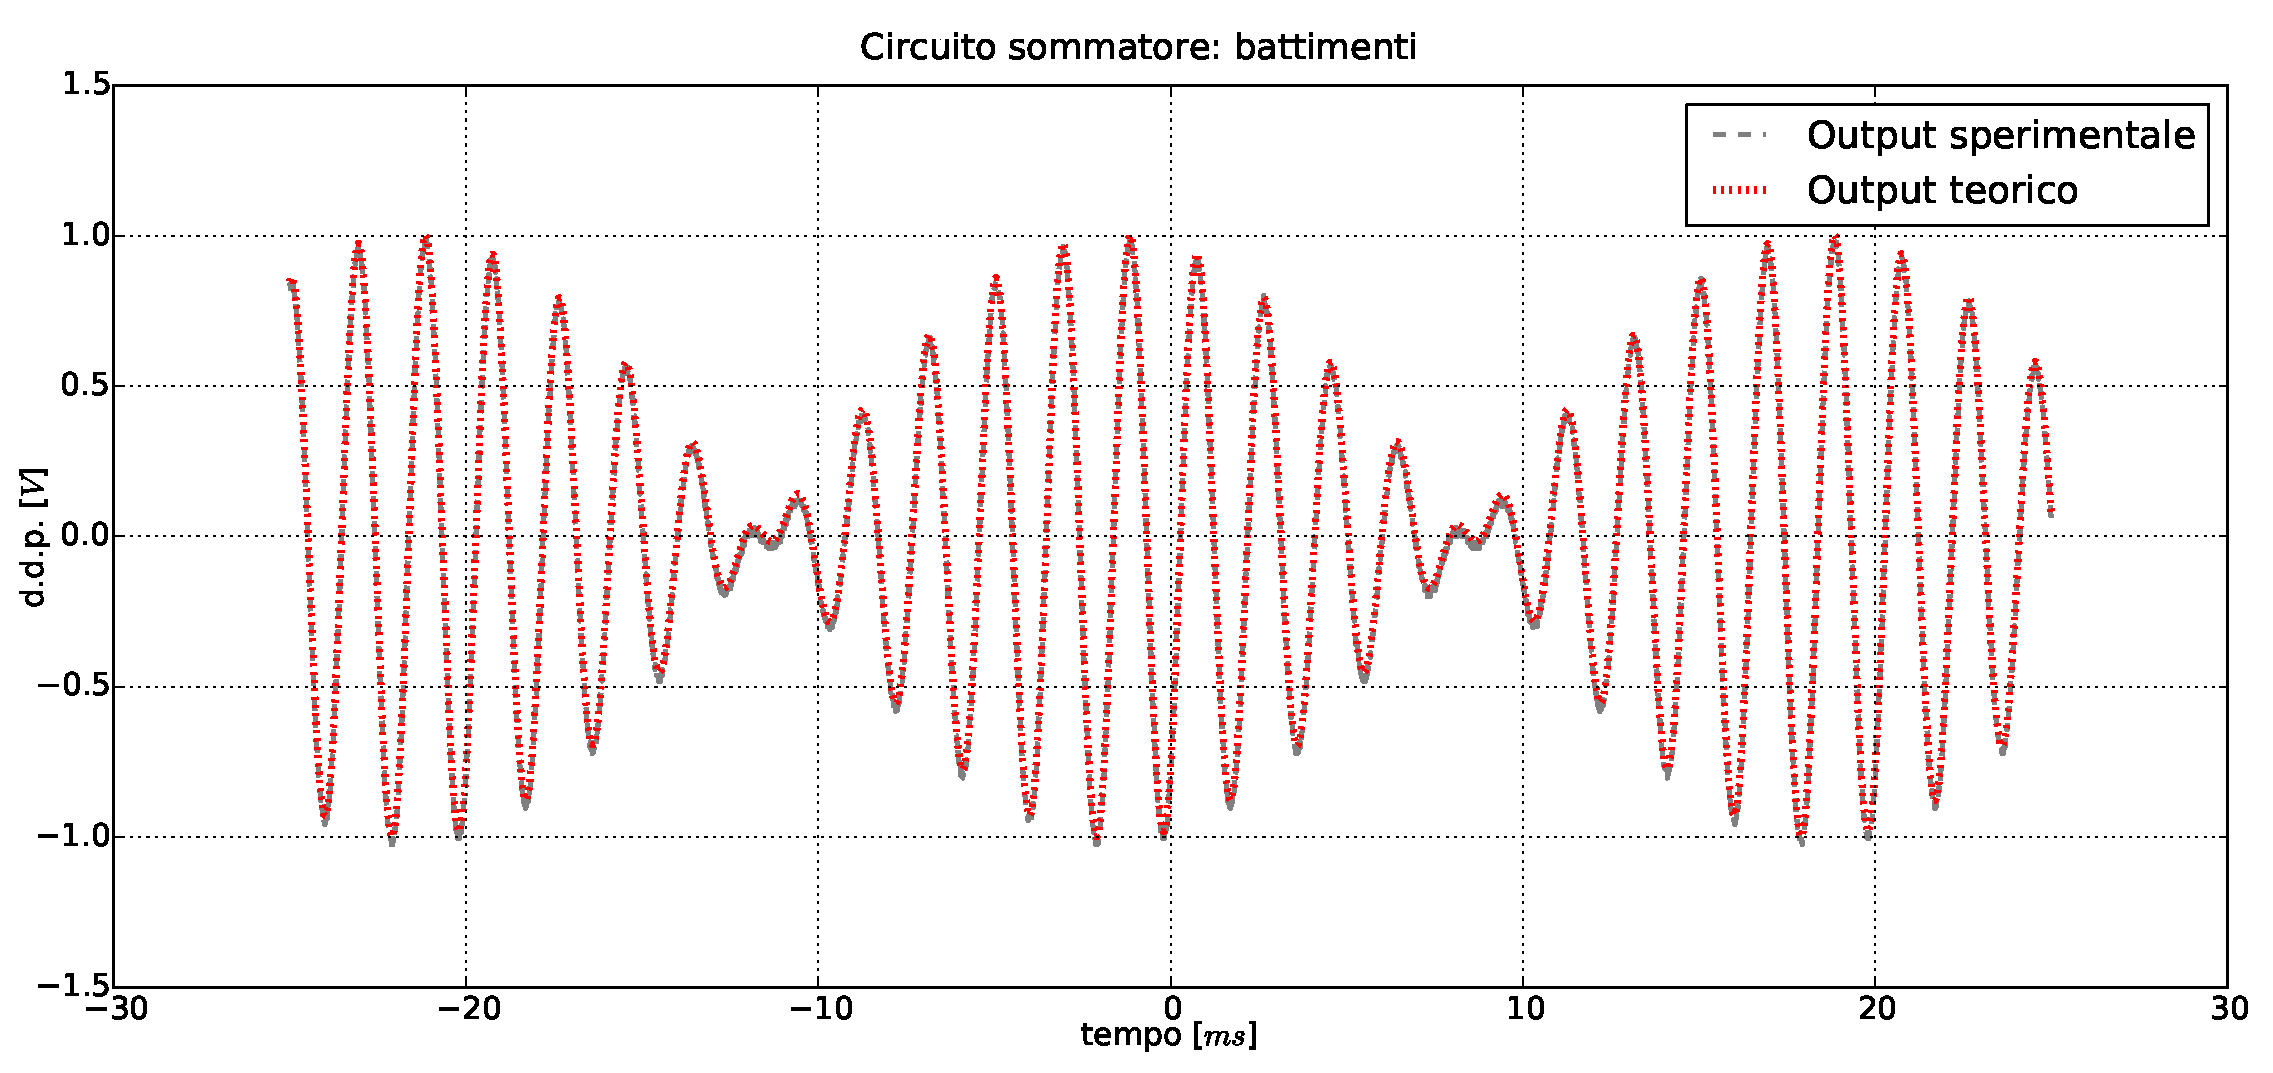
\includegraphics[width=18cm]{../E01/latex/battimenti_ideali.pdf}}
 \caption{...}
 \label{gr:onde1}
\end{figure}



\begin{figure}[H]
 \centering
   {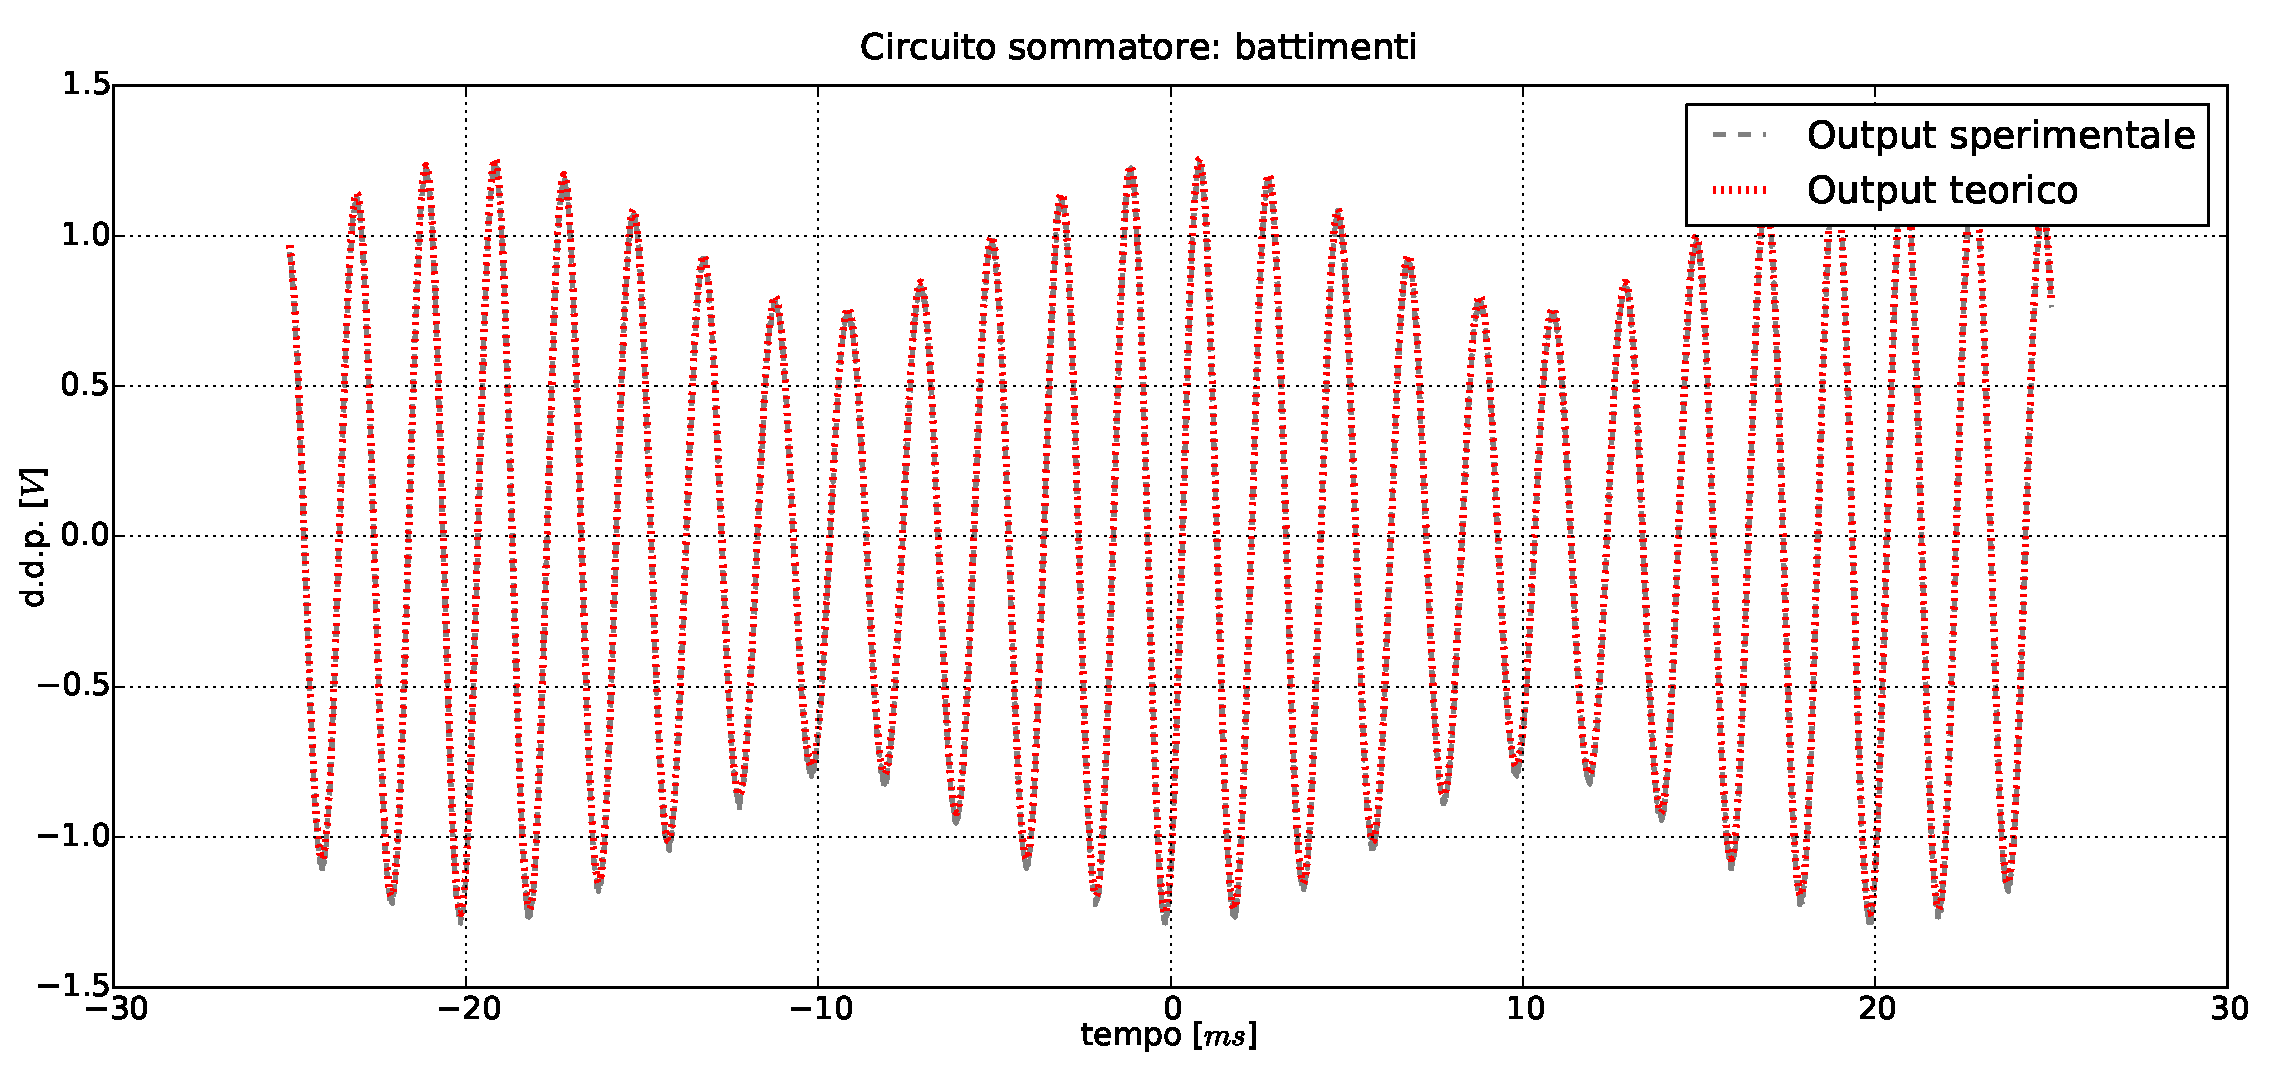
\includegraphics[width=18cm]{../E01/latex/battimenti.pdf}}
 \caption{...}
 \label{gr:onde1}
\end{figure}















